


\begin{figure}[H]
\centering
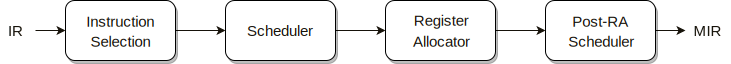
\includegraphics[width=.15\textwidth]{figures/phase_ordering}
\caption{General code generation phases.}
\label{fig:phase_ordering}
\end{figure}

%Approach 1
Post RA pass to allocate bypass sources by demoting operands to bypass registers where possible.
When a bypass is allocated, it replaces the register that it used to take as operand, therefore effectively freeing a register. However in the post-RA stage, spill code has already been inserted, this will not benefit in terms of freeing registers, unless we move spill code explicitly. This will be be the easiest approach, because even without moving the spill code, this method will still work, but with too early inserted spill code as a result.

%Approach 2
Bypass-aware register allocator that allocates bypass sources as much as possible, and then allocates any virtual registers not bypass as any normal register allocator. In this approach the freed registers can be utilized which should give overall better results.

%Approach 3
If we allocate bypasses after scheduling, but before register allocation, we can change a virtual register into a bypass register when possible. However, during register allocation or any other passes that follow, code might be inserted that break a previously allocated bypass. For this reason, we will need another pass that will identify these broken bypasses, and change them back into virtual registers so that they are dealt with by the register allocator.

%Approach 4
Before scheduling, we can identify instruction pairs that we can bypass. Then we change the virtual register that is bypassed into physical (bypass) registers and glue the two instructions together. This way the scheduler will try to keep them together, and if it fails to do so, we might need to undo this bypass allocation in order to ensure that the program still works correctly.


%Approach 5
Implement a bypass-aware combined scheduler and register allocator.


%%%%%%%%%%%%%%%%%%%%%%%%%%%%%%%%%%

In Chapter \ref{sec:processor} we have briefly discussed the bypassing sources of the proposed architecture. For convenience we have given them again in Table \ref{table:bypass_alias}.

\begin{table}[H]
\caption{Alias for each bypassing source, $BP\_src$ in Figure \ref{fig:4_stage} and Figure \ref{fig:5_stage}.}
\begin{center}
\begin{tabular}{@{}llll@{}}
\toprule
\multirow{2}{*}{\textbf{Register:}} & \multirow{2}{*}{\textbf{Bypass source:}} & \multicolumn{2}{c}{\textbf{Alias}:} \\ \cline{3-4}
 & & \textbf{4 stages} & \textbf{5 stages} \\
\hline
\emph{r27} & $BP\_src27$ & N/A & ALU1 \\ 
\emph{r28} & $BP\_src28$ & LSU & LSU \\
\emph{r29} & $BP\_src29$ & MUL & MUL \\ 
\emph{r30} & $BP\_src30$ & ALU & ALU2 \\
\emph{r31} & $BP\_src31$ & WB & WB \\
\bottomrule
\end{tabular}
\end{center}
\label{table:bypass_alias}
\end{table}%



Proposed solutions: phase ordering problem, discuss each possible implementation here, ordered by difficulty. Indicate that in the available timespan, we can not implement all of these solutions.
